\section{All chambers}\label{app:allchambers}
\intent{The main text follows chamber~A. These are the same measurements for every chamber, to show what varies from one
board to the next (Dylan 2026-11-03).}

\begin{figure}[h]
  \centering
  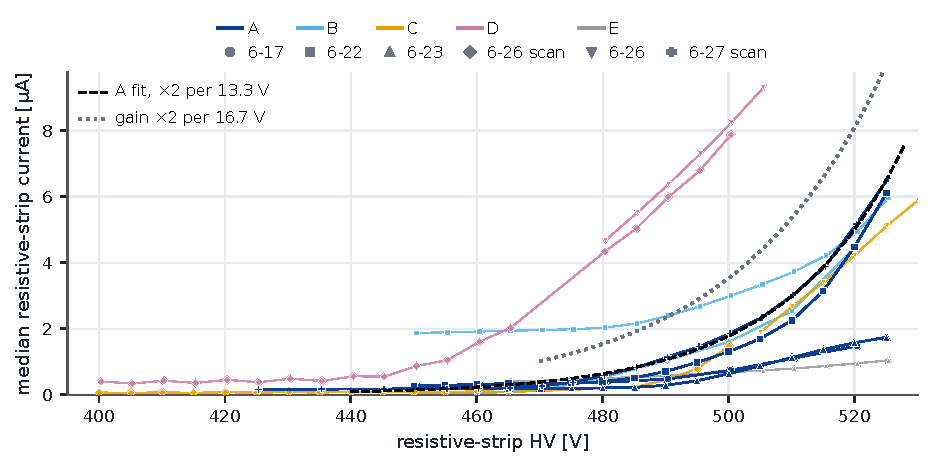
\includegraphics[width=\linewidth]{currents_vs_hv_all}
  \caption{\tbw{Resistive-electrode current against HV for every board, from 17 June on. Colour: chamber; marker: night (``scan'': HV-scan days; other dates: overnight runs). Dashed: the chamber~A fit $I=1.05\,\text{\textmu A}\times2^{(V-490\,\text{V})/13.3\,\text{V}}$; dotted: one gain doubling per 16.7\,V, for reference. Linear scale.}}
  \label{fig:currents_all}
\end{figure}

\begin{figure}[h]
  \centering
  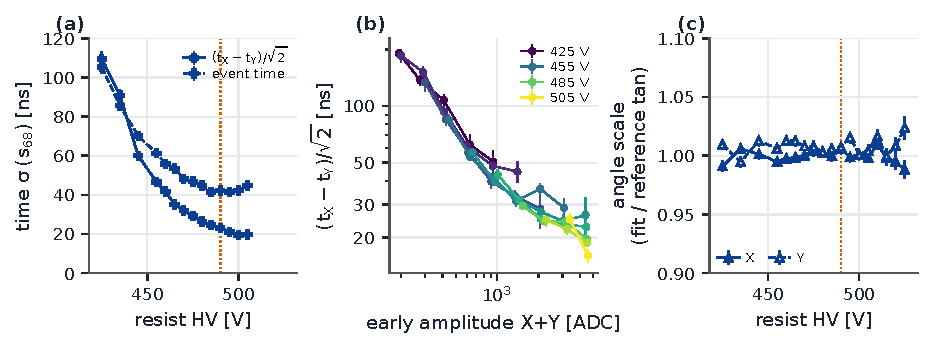
\includegraphics[width=\linewidth]{hv_metrics_extra}
  \caption{\tbw{Chamber~A against the resist HV (6-27 scan), the two quantities left out of \cref{fig:hvmetrics}. (a) Time resolution: the uncorrelated part $(t_X-t_Y)/\sqrt2$ (filled) and the event time (open), not measured above 505\,V. (b) The uncorrelated part against the early amplitude (strip sum at the rising-edge cut, $X+Y$), one curve per HV step (selected steps shown): every HV lies on the same curve, so the improvement with HV is the signal-to-noise of the edge estimate, not a change of the chamber. (c) Angle scale (slope of the fitted against the reference $\tan$); X filled, Y open. Dotted vertical line: 490\,V.}}
  \label{fig:hvmetrics_extra}
\end{figure}

\begin{figure}[h]
  \centering
  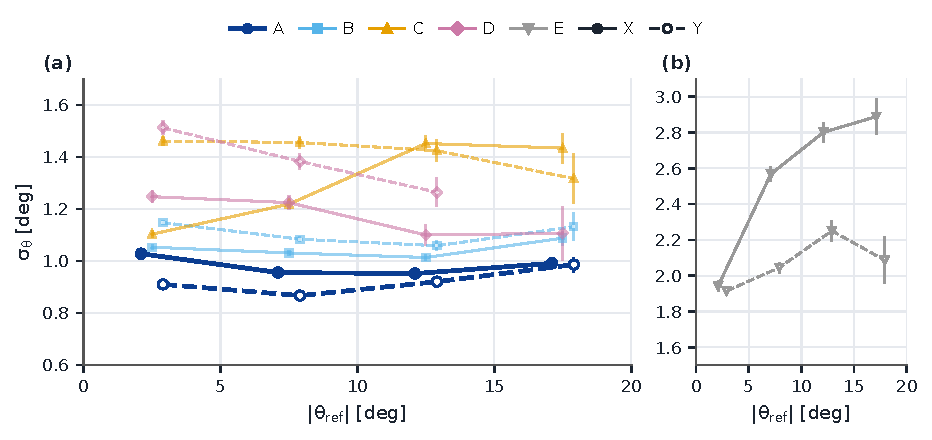
\includegraphics[width=\linewidth]{tracking_perf_all}
  \caption{\tbw{Angular resolution $\sigma_\theta$ (the $s_{68}$ of $\theta_\mathrm{fit}-\theta_\mathrm{ref}$, interior tracks matched to the reference) against $|\theta_\mathrm{ref}|$ in 5\textdegree{} bins, X (solid, filled) and Y (dashed, open) of each chamber. (a) Chambers A to D; A is Runs 1 and 2 summed, the others their golden runs (the calibration runs for C and D, hence in-sample). (b) Chamber~E on its own scale. Error bars $s_{68}/\sqrt{2n}$; bins with fewer than 50 tracks are omitted.}}
  \label{fig:trackperf_all}
\end{figure}

\begin{figure}[h]
  \centering
  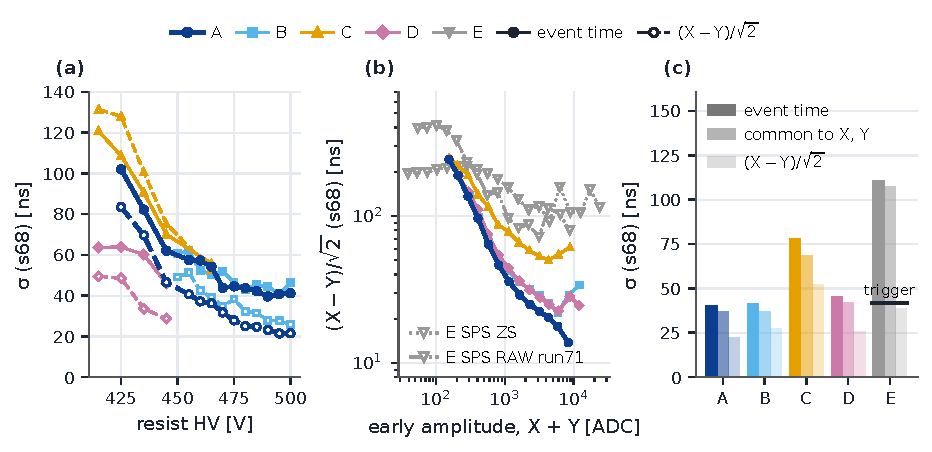
\includegraphics[width=\linewidth]{timing_all}
  \caption{\tbw{Time resolution on the bench for all chambers: (a) event time (solid) and uncorrelated part (dashed) against the resist HV in the scans; (b) the uncorrelated part against the signal size, with chamber~E at SPS (open grey); (c) on the golden runs, the event time, the part common to X and Y, and the uncorrelated part. The trigger term is 42\,ns (chamber~E).}}
  \label{fig:timing_all}
\end{figure}
